
\documentclass[a4paper,12pt]{article}

\usepackage[font=scriptsize]{caption}
\usepackage{mwe}
\newcommand\tab[1][1cm]{\hspace*{#1}}


\usepackage{booktabs}
\usepackage{tikz}
\usepackage{amsmath,amssymb,amsthm,enumitem, amsfonts,listings,upquote, graphicx, color}
\usepackage[document]{ragged2e} %left justifies everything automatically
\usepackage{algorithm, algpseudocode}

% \usepackage{algorithm}
% \usepackage[noend]{algpseudocode}

\usepackage{fancyref}
\usepackage{color} %red, green, blue, yellow, cyan, magenta, black, white


\usepackage{adjustbox}
\usepackage{ifthen}

\usepackage{CJK}
\usepackage{comment}
\usepackage{varioref}

\usepackage[nottoc]{tocbibind}
 

\excludecomment{mysection}


\DeclareMathOperator{\prox}{\mathbf{prox}}
\DeclareMathOperator*{\argmin}{arg\,min}

\newcommand{\N}{\mathbb{N}}
\newcommand{\Z}{\mathbb{Z}}

\newcommand\norm[1]{\left\lVert#1\right\rVert}
\makeatletter
\def\BState{\State\hskip-\ALG@thistlm}
\makeatother

\algdef{SE}[DOWHILE]{Do}{doWhile}{\algorithmicdo}[1]{\algorithmicwhile\ #1}%

\lstset{ 
  tabsize=1,
  showstringspaces=false,
  breaklines=true,
}

%\addtolength{\oddsidemargin}{-.875in}
%\addtolength{\evensidemargin}{-.875in}
%\addtolength{\textwidth}{1.75in}
%\addtolength{\topmargin}{-.875in}
%\addtolength{\textheight}{1.75in}

\definecolor{mygreen}{RGB}{28,172,0} % color values Red, Green, Blue
\definecolor{mylilas}{RGB}{170,55,241}

\makeatletter
\newcommand{\thickhline}{%
    \noalign {\ifnum 0=`}\fi \hrule height 1pt
    \futurelet \reserved@a \@xhline
}

\newcommand{\sthickhline}{%
    \noalign {\ifnum 0=`}\fi \hrule height 0.1pt
    \futurelet \reserved@a \@xhline
}

\usepackage{blindtext}
\title{Predicting Survival on Titanic}
\author{Carrie Lei\\ (415)810-8610\\leoi06012015@gmail.com} \date{\today}


\begin{document}
\maketitle

\justify

\begin{section}{Abstract}
% Goal
The goal for this project is to build a mathematical model to predict survival
of passengers on Titanic given the information of their ages, passenger class,
gender, etc. Data are retrieved through online website Kaggle.




\end{section}


\begin{section}{Analyzing data}
There are two sets of data, one for training the model and the other one for testing the performance of the model.\\
First step is to understand what the data means.  \\
\begin{comment}
Python code: \\
train $=$ pd.read\_csv('titanic\_train.csv')\\
train.head()\\



% table_head
\end{comment}

\begin{figure}
% heatmap
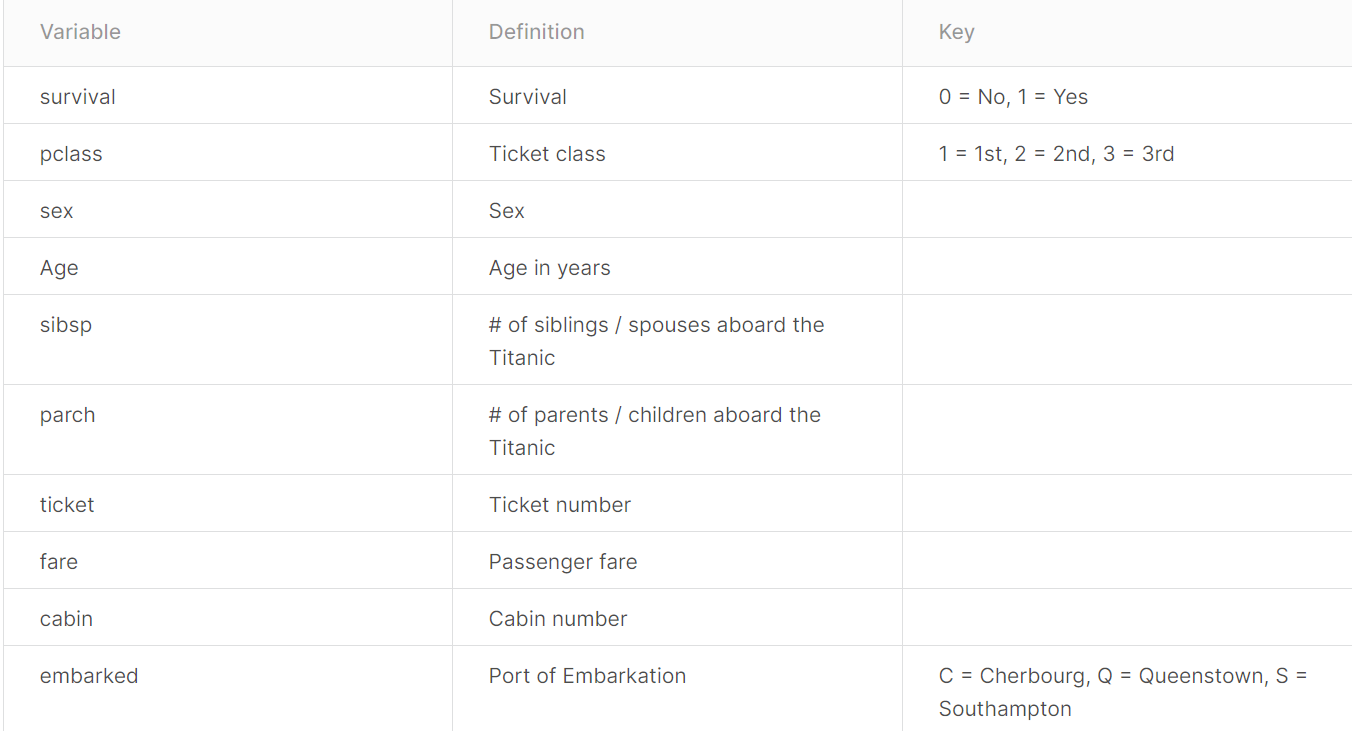
\includegraphics[scale=0.5]{titanice_data_preview.png}\\
	\caption{Description of the data.}
\end{figure}

\begin{figure}
% heatmap
  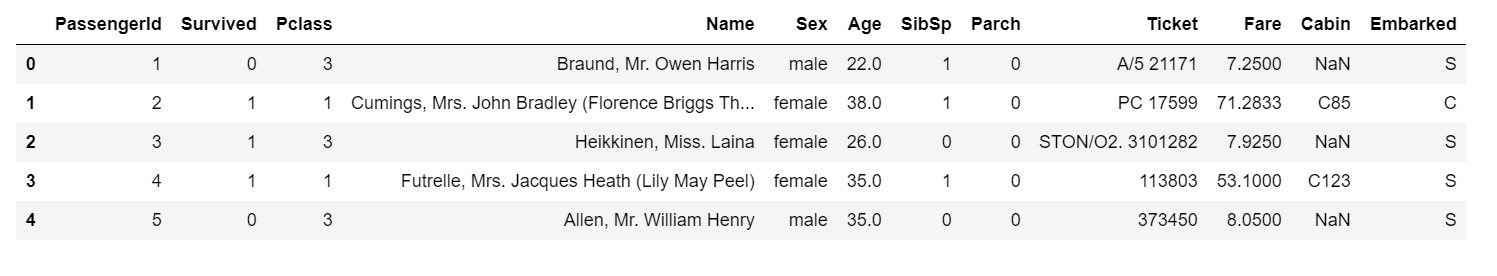
\includegraphics[width=\textwidth]{table_head.png}
	\caption{First 5 columns of the data set.}
\end{figure}




Next, I tried to explore the data by visualizing them.\\


\begin{figure}
\centering
\begin{minipage}{.5\textwidth}
  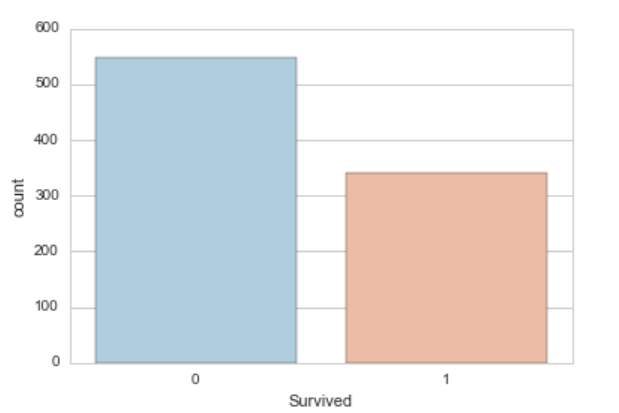
\includegraphics[width=\textwidth]{survive_Ratio.png}
  \caption{Count survival situation (0 represents not survived and 1 represents survived).}
\end{minipage}%
\hfill
\begin{minipage}{.5\textwidth}
  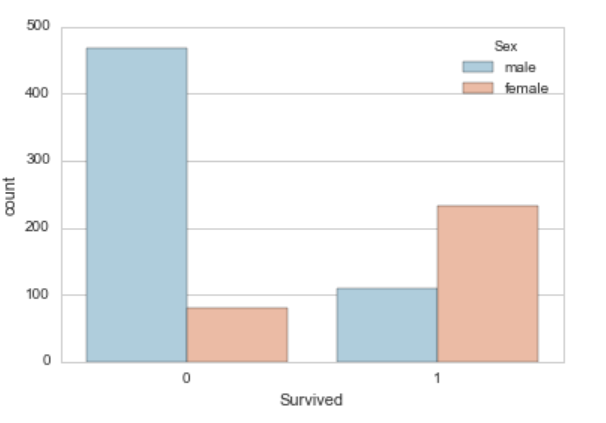
\includegraphics[width=\textwidth]{gender_survive.png}
  \caption{Count the number of different gender in each survival situation.}
\end{minipage}
\end{figure}



\begin{figure}
\centering
\begin{minipage}{.5\textwidth}
  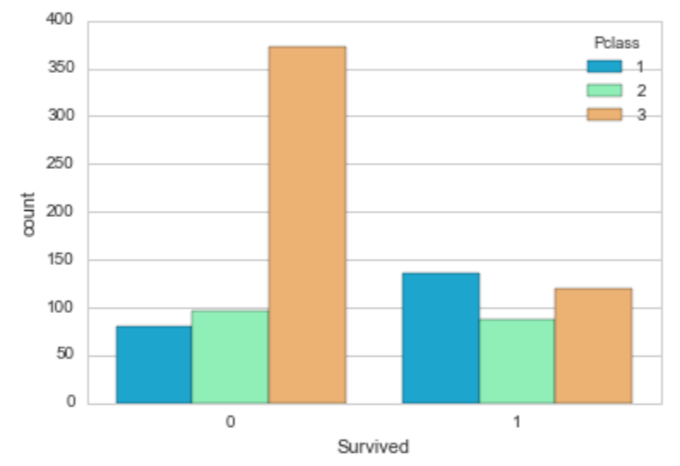
\includegraphics[width=\textwidth]{pclass_survive.png}
  \caption{Count survival situation (0 represents not survived and 1 represents survived).}
\end{minipage}%
\hfill
\begin{minipage}{.5\textwidth}
  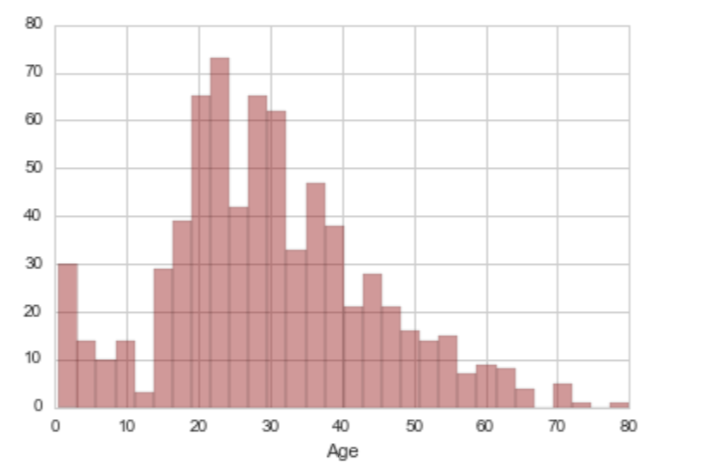
\includegraphics[width=\textwidth]{age.png}
  \caption{Count the number of different gender in each survival situation.}
\end{minipage}
\end{figure}


\begin{figure}
% heatmap
  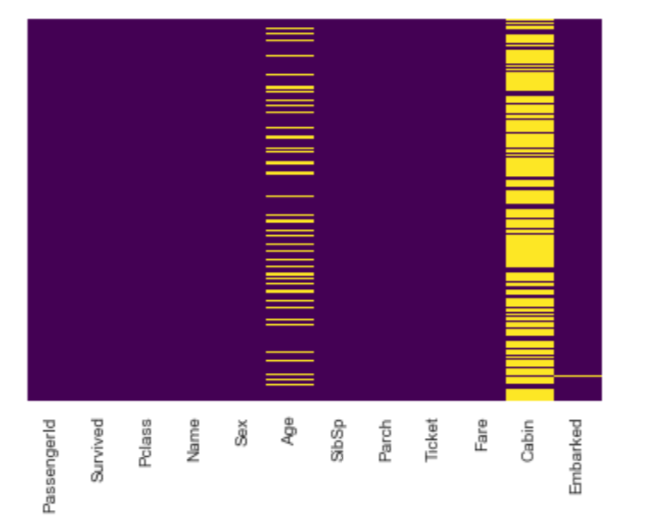
\includegraphics[width=\textwidth]{heatmap.png}
	\caption{Heatmap to visualize what data is missing.}
\end{figure}

% where did I got the data
% what each colomn means

\end{section}


\begin{section}{Cleaning the data}
As we can notice from the data above, some age data are missing. I would be nice to fill in the missing data by approximating them. Instead of fill in the average age of the whole data set, I separated  the data by their passenger class and find the average age of each class and fill in the average age according to the class that the data belong to. \\

For the cabin data, since so many data are missing, I just dropped the whole column of data. I also dropped the name column and ticket column, since they do not matter.

\begin{figure}
% heatmap
  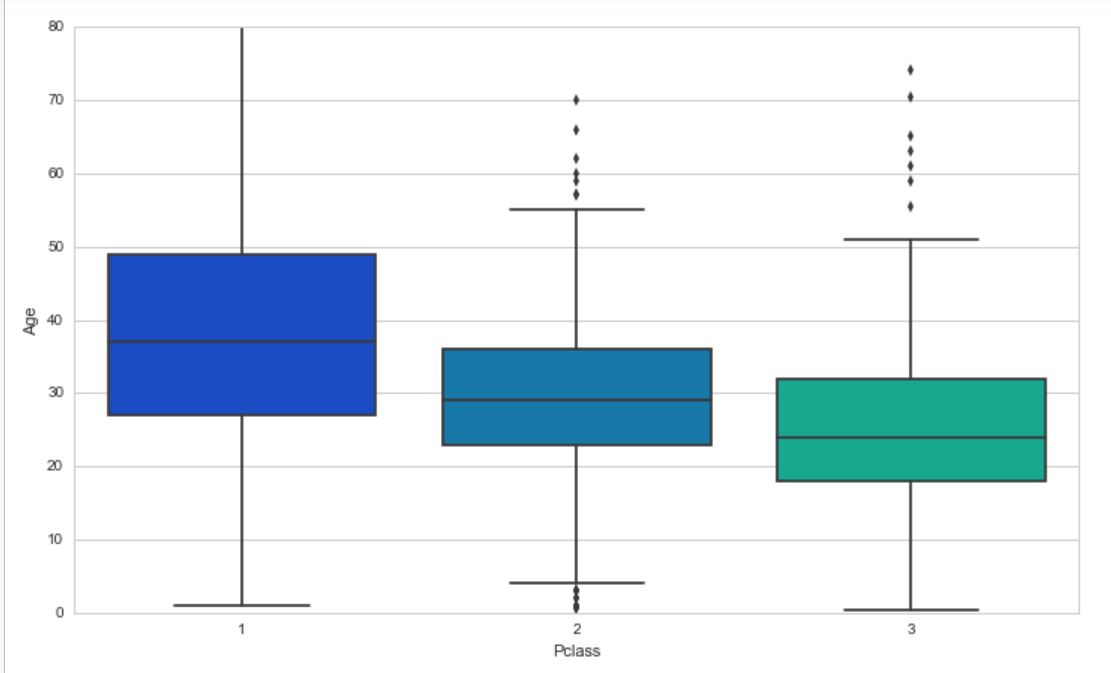
\includegraphics[width=\textwidth]{age_pclass.png}
	\caption{Box plot of age for each class.}
\end{figure}

As we can see, some data are categorical data and it would be nice to convert them into numerical data. For gender data, I use 1 or 0 to represent whether the passenger is male or female. For Embark column, I used the same method to keep track of whether the passenger embarked at Q, S or neither (which means C). 

\begin{figure}
% heatmap
  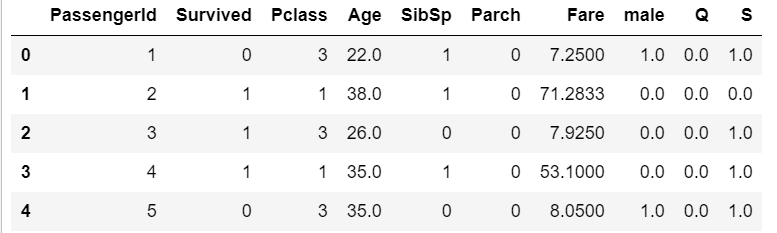
\includegraphics[width=\textwidth]{converted_data.png}
	\caption{Converted data.}
\end{figure}
% converted_data

% method I used to clean the Age column
% ignore column that miss too many data
% convert the catergorical data into numerical data
\end{section}

\begin{section}{Train the Model}

Since I know the data that represent whether the passenger survived or not is a binary data, so I used the Logistic Regression model to train the data.
% split the data and train them
Python code:

 from sklearn.linear\_model import LogisticRegression\\
\tab logmodel $=$ LogisticRegression()\\
\tab logmodel.fit(X\_train,y\_train)\\



\end{section}

\begin{section}{Evaluate the Model}
After I got the trained model, I used the test data to evaluate the performance of the model by compare the actual value from the test data and the predict values from the model.
Python Code:
from sklearn.metrics import classification\_report\\



\begin{figure}
% heatmap
  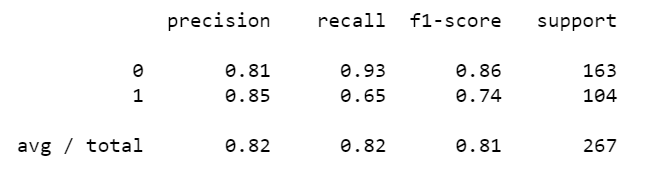
\includegraphics[width=\textwidth]{result.png}
	\caption{Model performance evaluation.}
\end{figure}

Denote TP as number of True Positive, TN as True Negative, FP as False Positive, FN as False Negative.
Where $precision = \frac{TP}{TP + FN }$, $ Recall = \frac{TP}{TP + FN}$, $F1_score = 2*(Recall * Precision) / (Recall + Precision)$, support  is the number of occurrences of each class in the test data.

\end{section}

\begin{section}{Conclusion}
% split the data and train them
The success rate to predict the survival of a passenger by this model is 82\%.
\newpage
\end{section}
\begin{section}{Reference Python Code}
\begin{lstlisting}
import pandas as pd
import numpy as np
import matplotlib.pyplot as plt
import seaborn as sns
# import tensorflow as tf


train = pd.read_csv('train.csv')

# plt.subplot(2, 2, 1)
# sns.heatmap(train.isnull(), yticklabels=False, cbar=False, cmap='viridis')
#
# plt.subplot(2, 2, 2)
# sns.set_style('whitegrid')
# sns.countplot(x='Survived',data=train,palette='RdBu_r')
#
# plt.subplot(2, 2, 3)
# sns.countplot(x='Survived',hue='Sex',data=train,palette='RdBu_r')
#
# plt.subplot(2,2,4)
# sns.countplot(x='Survived',hue='Pclass',data=train,palette='rainbow')

# sns.distplot(train['Age'].dropna(),kde=False,color='darkred',bins=30)
# plt.show()

# plt.figure(figsize=(10, 5))
# sns.boxplot(x='Pclass',y='Age',data=train,palette='summer')
# plt.show()

# calculate the average age for each passenger class
Class = train['Pclass']
# print(Class)
train_test = train.dropna(subset=['Age'])
# print(train_test.head(5))

class1_mean = train_test[train_test['Pclass'] == 1]['Age'].mean()
# print(class1_mean)
class2_mean = train_test[train_test['Pclass'] == 2]['Age'].mean()
# print(class2_mean)
class3_mean = train_test[train_test['Pclass'] == 3]['Age'].mean()
# print(class3_mean)

def replace_null(cols):
    Pclass = cols[0]
    Ages = cols[1]
    if pd.isnull(Ages):
        if Pclass == 1:
            return class1_mean
        if Pclass == 2:
            return class2_mean
        if Pclass == 3:
            return class3_mean

    else:
        return Ages


train['Age'] = train[['Pclass', 'Age']].apply(replace_null, axis=1)


sns.heatmap(train.isnull(),yticklabels=False,cbar=False,cmap='viridis')


train.drop('Cabin', axis=1, inplace=True)
sex = pd.get_dummies(train['Sex'], drop_first=True)
embark = pd.get_dummies(train['Embarked'], drop_first=True)
train.drop(['Sex', 'Embarked', 'Name', 'Ticket'], axis=1, inplace=True)
train = pd.concat([train, sex, embark], axis=1)
print(train.head(3))
# plt.show()


\end{lstlisting}

\end{section}

\end{document}